\section{Online Recover Procedure} \label{sec:online}
%
With the support of hardware architecture and offline program transformer, this section presents the online recover procedure, including the reconfiguration (Sec.~\ref{sec:onlineReconfig}) and the restart (Sec.~\ref{sec:onlineRestart}) of peripherals.






\subsection{Peripheral Operation Restart} \label{sec:onlineRestart}
%\vspace{-5pt}
%
After the peripherals are reconfigured, we are ready to restart the peripheral operations.
REMARK restarts the peripheral operations from peripheral checkpoints with the help of PRM (described in Sec.~\ref{sec:hardware}) and Initiator.



%\vspace{5pt}
\noindent\textbf{The Restart Flows after Power Failure.} \\
The restart flows are different from each other when power fails during different stages.
A peripheral operation can be decomposed into three stages: the starting stage, the execution stage, and the returning stage.
During the starting stage, the processor uses I/O instructions to start a peripheral operation.
The execution stage lasts until the returning interrupt is triggered.
Finally, the ISR returns the result to the processor in the returning stage.
The peripheral operation is completed only if the ISR is finished.

%
When power fails during the starting stage, the parallel peripheral operation has not been started.
No peripheral checkpoints are placed, and the processor only needs to rollback and re-run the starting stage.
Once the starting stage is completed, \emph{updateInitiator()} inserted during offline program transformation will place a peripheral checkpoint in Initiator.

When power fails during the execution stage, as shown in Fig.~\ref{fig:PeriRecoverProcedure} (a), the processor restores its state and the peripheral operations are restarted from their checkpoints individually.

When power fails during the returning stage, as shown in Fig.~\ref{fig:PeriRecoverProcedure} (b), the peripherals lose all the data and fail to return the results.
Therefore, the peripheral operations still need to be restarted.
Meanwhile, the processor needs to restore to the checkpoint located before the ISR, as discussed in Sec.~\ref{sec:offlineTransformer}.
When a successful ISR is completed, the peripheral operation is also finished.
Therefore, the peripheral checkpoint to restart this operation needs to be removed from Initiator by another \emph{\_updateInitiator()} function.

%
\begin{figure}[t]
    \centering
    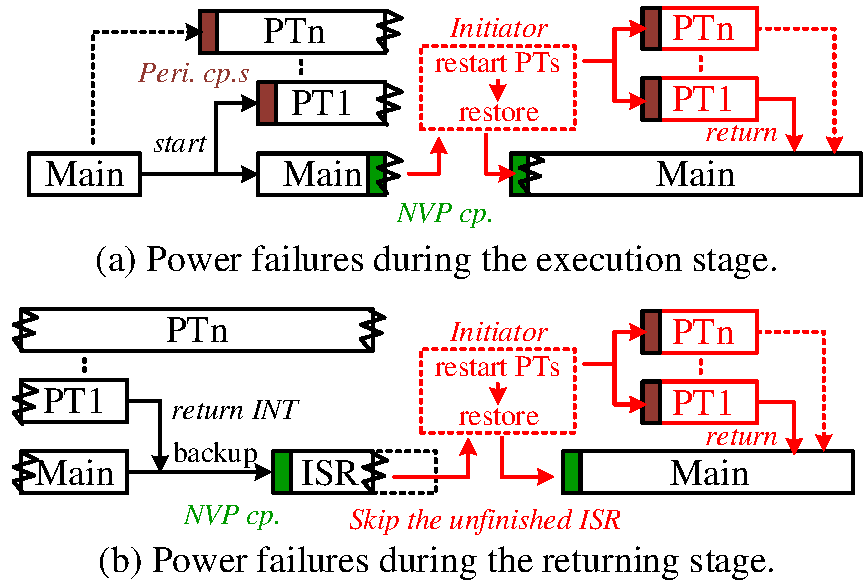
\includegraphics[width=0.45\textwidth]{Fig10_PeriRecoverProcedure.pdf}
    %\vspace{-5pt}
    \caption{Power failures during the starting and the returning stage of peripheral operations.}
    %\vspace{-5pt}
    \label{fig:PeriRecoverProcedure}
\end{figure}

% the resilience of REMARK
When power fails during the recover procedure, the devices can roll back to their checkpoints if these checkpoints are not crashed.
Therefore, completing the backup function is essential to ensure the validity of a checkpoint.
To guarantee the success of backup operation, NVP adopts a $4.7 \mu F$ on-chip capacitor.
In the hardware prototype of this paper, each backup operation consumes $77.69nJ$ in $7 \mu s$.
In this way, the system can safely backup whenever power fails.
